\documentclass{beamer}
\usepackage[utf8]{inputenc}
\usepackage[spanish]{babel}
\usetheme{Goettingen}
\usecolortheme{default}
\useoutertheme{shadow}
\useinnertheme{rectangles}
\graphicspath{ {./figures/} }
\title[Laboratorio]{Introducción}
\subtitle{Herramientas de trabajo}
\author[Miguel]{Miguel Angel Piña Avelino}
\institute[UNAM]{
  Facultad de Ciencias, UNAM
}
\AtBeginSection[]{
  \begin{frame}
  \vfill
  \centering
  \begin{beamercolorbox}[sep=8pt,center,shadow=true,rounded=true]{title}
    \usebeamerfont{title}\insertsectionhead\par%
  \end{beamercolorbox}
  \vfill
  \end{frame}
}


\date{\today}

\begin{document}

\frame{\titlepage}

\begin{frame}
  \frametitle{Índice}
  \tableofcontents
\end{frame}

\section{Cuestionario}

\begin{frame}
  \frametitle{Cuestionario}
  https://goo.gl/forms/IHatNs24nUIfiOhl2
\end{frame}

\section{Introducción}

\begin{frame}[fragile]
  \frametitle{Repositorio}
  El material que revisemos en el laboratorio va a estar disponible en
  la siguiente dirección:
\begin{verbatim}
https://github.com/miguelpinia/ingenieria-de-software
\end{verbatim}
\end{frame}

\begin{frame}
  \frametitle{Introducción}
  Las herramientas más importantes del curso que usaremos serán:
  \begin{itemize}
    \item Java EE 8
    \item Netbeans 8.2
    \item Git
    \item PostgreSQL
  \end{itemize}
\end{frame}

\section{Java EE}

\begin{frame}
  \frametitle{¿Qué es Java EE?}
  Java Platform, Enterprise Edition o Java EE (anteriormente conocido
  como Java 2 Platform, Enterprise Edition o J2EE hasta la versión
  1.4; traducido informalmente como Java Empresarial), es una
  plataforma de programación—parte de la Plataforma Java—para
  desarrollar y ejecutar software de aplicaciones en el lenguaje de
  programación Java.
\end{frame}

\begin{frame}
  \frametitle{¿Qué es Java EE?}
  Permite la creación de arquitecturas de N capas distribuidas y se
  apoya en componentes modulares que se ejecutan sobre un servidor de
  aplicaciones (servlet container).

  \begin{figure}[ht]
    \centering
    
\includegraphics[scale=0.25]{figures/javaee1.png}
    \caption{\label{fig:javaee1}Logotipo de Java EE}
  \end{figure}
\end{frame}

\begin{frame}
  \frametitle{Usos de Java EE}

  \begin{itemize}
    \item Está orientado a empresas y a la integración entre sistemas.
    \item Incluye soporte a tecnologías para internet.
    \item Su base es Java SE.\@
  \end{itemize}
\end{frame}

\begin{frame}
  \frametitle{Características}
    Algunas de sus funcionalidades más importantes son:
  \begin{itemize}
    \item Acceso a base de datos (JDBC)
    \item Utilización de directorios distribuidos (JNDI)
    \item Acceso a métodos remotos (RMI/CORBA)
    \item Funciones de correo electrónico (JavaMail)
    \item Aplicaciones Web (JSP y Servlet)
    \item Uso de Beans, etc.
  \end{itemize}
\end{frame}

\begin{frame}
  \frametitle{Características}
    Algunas de sus funcionalidades más importantes son:
  \begin{itemize}
    \item \textbf{Acceso a base de datos (JDBC)}
    \item Utilización de directorios distribuidos (JNDI)
    \item Acceso a métodos remotos (RMI/CORBA)
    \item Funciones de correo electrónico (JavaMail)
    \item Aplicaciones Web (JSP y Servlet)
    \item Uso de Beans, etc.
  \end{itemize}
\end{frame}

\begin{frame}
  \frametitle{JDBC}
  \textbf{Java Database Connectivity}, más conocida por sus siglas
  \textbf{JDBC}, es una API que permite la ejecución de operaciones
  sobre bases de datos desde el lenguaje de programación Java,
  independientemente del sistema operativo donde se ejecute o de la base
  de datos a la cual se accede, utilizando el dialecto SQL del modelo de
  base de datos que se utilice.
\end{frame}

\begin{frame}
  \frametitle{Características}
    Algunas de sus funcionalidades más importantes son:
  \begin{itemize}
    \item Acceso a base de datos (JDBC)
    \item \textbf{Utilización de directorios distribuidos (JNDI)}
    \item Acceso a métodos remotos (RMI/CORBA)
    \item Funciones de correo electrónico (JavaMail)
    \item Aplicaciones Web (JSP y Servlet)
    \item Uso de Beans, etc.
  \end{itemize}
\end{frame}

\begin{frame}
  \frametitle{JNDI}
  La Interfaz de Nombrado y Directorio Java (\textbf{Java Naming and
    Directory Interface}) es una Interfaz de Programación de Aplicaciones
  (API) de Java para servicios de directorio. Permite a los clientes
  descubrir y buscar objetos y datos a través de un nombre. Como todas
  las APIs de Java que hacen de interfaz con sistemas host, es
  independiente de la implementación subyacente.
\end{frame}


\begin{frame}
  \frametitle{Características}
    Algunas de sus funcionalidades más importantes son:
  \begin{itemize}
    \item Acceso a base de datos (JDBC)
    \item Utilización de directorios distribuidos (JNDI)
    \item \textbf{Acceso a métodos remotos (RMI/CORBA)}
    \item Funciones de correo electrónico (JavaMail)
    \item Aplicaciones Web (JSP y Servlet)
    \item Uso de Beans, etc.
  \end{itemize}
\end{frame}

\begin{frame}
  \frametitle{RMI/Corba}
  RMI ("Remote Method Invocation") y algunas alternativas como CORBA y
  COM son mecanismos para invocar ó ejecutar procedimientos remotos en
  computadoras ó servidores distribuidos.
\end{frame}

\begin{frame}
  \frametitle{Características}
    Algunas de sus funcionalidades más importantes son:
  \begin{itemize}
    \item Acceso a base de datos (JDBC)
    \item Utilización de directorios distribuidos (JNDI)
    \item Acceso a métodos remotos (RMI/CORBA)
    \item \textbf{Funciones de correo electrónico (JavaMail)}
    \item Aplicaciones Web (JSP y Servlet)
    \item Uso de Beans, etc.
  \end{itemize}
\end{frame}

\begin{frame}
  \frametitle{JavaMail}
  JavaMail es una API Java que facilita el envío y recepción de e-mail
  desde código java a través de protocolos SMTP, POP3 y IMAP. JavaMail
  está integrado en la plataforma Java EE, pero también proporciona un
  paquete opcional para su uso en Java SE.
\end{frame}


\begin{frame}
  \frametitle{Características}
    Algunas de sus funcionalidades más importantes son:
  \begin{itemize}
    \item Acceso a base de datos (JDBC)
    \item Utilización de directorios distribuidos (JNDI)
    \item Acceso a métodos remotos (RMI/CORBA)
    \item Funciones de correo electrónico (JavaMail)
    \item \textbf{Aplicaciones Web (JSP y Servlet)}
    \item Uso de Beans, etc.
  \end{itemize}
\end{frame}

\begin{frame}
  \frametitle{Servlet}
  El servlet es una clase en el lenguaje de programación Java,
  utilizada para ampliar las capacidades de un servidor. Aunque los
  servlets pueden responder a cualquier tipo de solicitudes, éstos son
  utilizados comúnmente para extender las aplicaciones alojadas por
  servidores web, de tal manera que pueden ser vistos como applets de
  Java que se ejecutan en servidores en vez de navegadores web. Este
  tipo de servlets son la contraparte Java de otras tecnologías de
  contenido dinámico Web, como PHP y ASP.NET.

\end{frame}

\begin{frame}
  \frametitle{JSP}
  JavaServer Pages (JSP) es una tecnología que ayuda a los
  desarrolladores de software a crear páginas web dinámicas basadas en
  HTML y XML, entre otros tipos de documentos. JSP es similar a PHP,
  pero usa el lenguaje de programación Java.

  Para desplegar y correr JavaServer Pages, se requiere un servidor web
  compatible con contenedores servlet como Apache Tomcat o Jetty.
\end{frame}

\section{Maven}

\begin{frame}
  \frametitle{¿Qué es Maven?}
  Es una herramienta de software para la gestión y construcción de
  proyectos en Java. Su funcionamiento es similar al de \textbf{Apache
    Ant}, pero va a tener un modo de configuración más simple, basado en
  un formato XML.
\end{frame}

\begin{frame}
  \frametitle{¿Qué es Maven?}
  Va a utilizar un Project Object Model (POM) para describir el proyecto
  de software a construir, dependencias a otros módulos y componentes
  externos, así como el orden de construcción de sus elementos.
\end{frame}

\begin{frame}
  \frametitle{¿QUé es Maven?}
  Una de las características claves de Maven es que está listo para
  trabajar en red, es decir, descargar todas las dependencias a través
  de repositorios de paquetes.
\end{frame}

\begin{frame}[fragile]
  \frametitle{Ejemplo de Maven}

  La forma más sencilla de crear un proyecto en Maven es:
\begin{verbatim}
mvn archetype:create -DgroupId="com.some.company" \
 -DartifactId="some-project" -Dversion="0.0.1"
\end{verbatim}

  Lo que va a generar un nuevo proyecto
\end{frame}

\begin{frame}[fragile]
  Una vez creado el proyecto, este va a tener la siguiente estructura:
  \begin{figure}[ht]
    \centering
    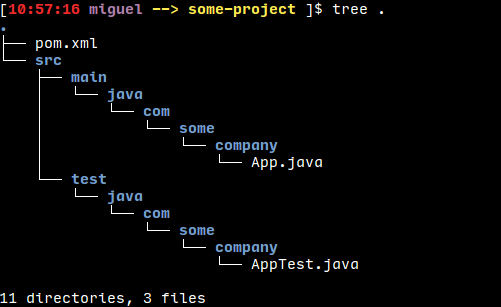
\includegraphics[scale=0.4]{figures/tree.png}
    \caption{\label{fig:tree} Árbol de directorios generados por Maven}
  \end{figure}

\end{frame}

\begin{frame}[fragile]
  El archivo pom.xml tiene el siguiente código generado.
  \begin{figure}[ht]
    \centering
    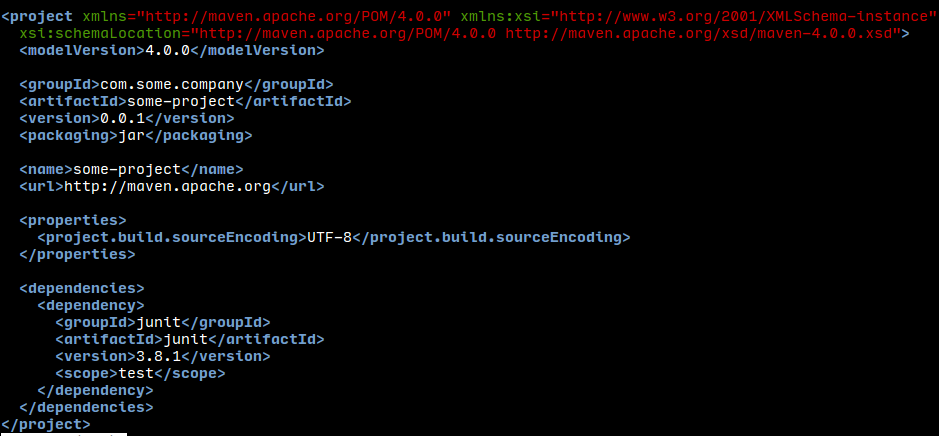
\includegraphics[scale=0.30]{figures/pom.png}
    \caption{\label{fig:pom} Contenido de un archivo pom.xml}
  \end{figure}

\end{frame}

\section{Netbeans}

\begin{frame}
  \frametitle{¿Qué es Netbeans?}
  \begin{itemize}
  \item IDE de código abierto
  \item Implementación de varios tipos de aplicaciones
    \begin{itemize}
    \item Aplicaciones de escritorio (Java SE)
    \item Aplicaciones web (Java Web)
    \item Aplicaciones empresariales (Java EE)
    \item Aplicaciones Móviles (Java ME)
    \end{itemize}
  \item Control de versiones (GIT, Mercurial, Subversion)
  \item Ant y Maven
  \end{itemize}
\end{frame}


\begin{frame}[fragile]
  \frametitle{Donde conseguir Netbeans}
  \begin{verbatim}
    https://netbeans.org/downloads/
  \end{verbatim}
\end{frame}

\section{GIT}

\begin{frame}
  \frametitle{¿Qué es GIT?}
  GIT es un software de control de versiones diseñado por Linus
  Torvalds, pensando en la eficiencia y la confiabilidad del
  mantenimiento de versiones de aplicaciones cuando estas tienen un
  gran número de archivos de código fuente.
\end{frame}

\begin{frame}[fragile]
  \frametitle{Tutorial de GIT}
  En internet hay varios tutoriales de GIT, pero este es uno de los que más me
  gustan:
  \begin{verbatim}
    https://try.github.io/levels/1/challenges/1
  \end{verbatim}
\end{frame}

\section{PostgreSQL}

\begin{frame}
  \frametitle{¿Qué es PostgreSQL?}
  PostgreSQL es un Sistema de gestión de bases de datos relacional orientado a
  objetos y libre, publicado bajo la licencia BSD.\\
  Actualmente se encuentra en la versión 10.1 la cual se publicó el 9
  de noviembre del 2017. Nosotros vamos a usar la versión \textbf{9.5}.
\end{frame}

\begin{frame}[fragile]
  \frametitle{¿Dónde lo consigo?}
  \begin{verbatim}
    http://www.postgresql.org/
  \end{verbatim}
\end{frame}

\end{document}
%%% Local Variables:
%%% mode: latex
%%% TeX-master: t
%%% End:
